\documentclass[french,]{article}
\usepackage{lmodern}
\usepackage{amssymb,amsmath}
\usepackage{ifxetex,ifluatex}
\usepackage{fixltx2e} % provides \textsubscript
\ifnum 0\ifxetex 1\fi\ifluatex 1\fi=0 % if pdftex
  \usepackage[T1]{fontenc}
  \usepackage[utf8]{inputenc}
\else % if luatex or xelatex
  \ifxetex
    \usepackage{mathspec}
  \else
    \usepackage{fontspec}
  \fi
  \defaultfontfeatures{Ligatures=TeX,Scale=MatchLowercase}
\fi
% use upquote if available, for straight quotes in verbatim environments
\IfFileExists{upquote.sty}{\usepackage{upquote}}{}
% use microtype if available
\IfFileExists{microtype.sty}{%
\usepackage[]{microtype}
\UseMicrotypeSet[protrusion]{basicmath} % disable protrusion for tt fonts
}{}
\PassOptionsToPackage{hyphens}{url} % url is loaded by hyperref
\usepackage[unicode=true]{hyperref}
\hypersetup{
            pdftitle={Rapport TP1 - Design Pattern},
            pdfauthor={Fleury Malik - malik.fleury@he-arc.ch; Wermeille Bastien - bastien.wermeille@he-arc.ch; Bulloni Lucas - lucas.bulloni@he-arc.ch},
            pdfborder={0 0 0},
            breaklinks=true}
\urlstyle{same}  % don't use monospace font for urls
\ifnum 0\ifxetex 1\fi\ifluatex 1\fi=0 % if pdftex
  \usepackage[shorthands=off,main=french]{babel}
\else
  \usepackage{polyglossia}
  \setmainlanguage[]{french}
\fi
\usepackage[top=3cm, bottom=2cm, left=2.5cm, right=3cm]{geometry}
\usepackage{color}
\usepackage{fancyvrb}
\newcommand{\VerbBar}{|}
\newcommand{\VERB}{\Verb[commandchars=\\\{\}]}
\DefineVerbatimEnvironment{Highlighting}{Verbatim}{commandchars=\\\{\}}
% Add ',fontsize=\small' for more characters per line
\newenvironment{Shaded}{}{}
\newcommand{\KeywordTok}[1]{\textcolor[rgb]{0.00,0.44,0.13}{\textbf{#1}}}
\newcommand{\DataTypeTok}[1]{\textcolor[rgb]{0.56,0.13,0.00}{#1}}
\newcommand{\DecValTok}[1]{\textcolor[rgb]{0.25,0.63,0.44}{#1}}
\newcommand{\BaseNTok}[1]{\textcolor[rgb]{0.25,0.63,0.44}{#1}}
\newcommand{\FloatTok}[1]{\textcolor[rgb]{0.25,0.63,0.44}{#1}}
\newcommand{\ConstantTok}[1]{\textcolor[rgb]{0.53,0.00,0.00}{#1}}
\newcommand{\CharTok}[1]{\textcolor[rgb]{0.25,0.44,0.63}{#1}}
\newcommand{\SpecialCharTok}[1]{\textcolor[rgb]{0.25,0.44,0.63}{#1}}
\newcommand{\StringTok}[1]{\textcolor[rgb]{0.25,0.44,0.63}{#1}}
\newcommand{\VerbatimStringTok}[1]{\textcolor[rgb]{0.25,0.44,0.63}{#1}}
\newcommand{\SpecialStringTok}[1]{\textcolor[rgb]{0.73,0.40,0.53}{#1}}
\newcommand{\ImportTok}[1]{#1}
\newcommand{\CommentTok}[1]{\textcolor[rgb]{0.38,0.63,0.69}{\textit{#1}}}
\newcommand{\DocumentationTok}[1]{\textcolor[rgb]{0.73,0.13,0.13}{\textit{#1}}}
\newcommand{\AnnotationTok}[1]{\textcolor[rgb]{0.38,0.63,0.69}{\textbf{\textit{#1}}}}
\newcommand{\CommentVarTok}[1]{\textcolor[rgb]{0.38,0.63,0.69}{\textbf{\textit{#1}}}}
\newcommand{\OtherTok}[1]{\textcolor[rgb]{0.00,0.44,0.13}{#1}}
\newcommand{\FunctionTok}[1]{\textcolor[rgb]{0.02,0.16,0.49}{#1}}
\newcommand{\VariableTok}[1]{\textcolor[rgb]{0.10,0.09,0.49}{#1}}
\newcommand{\ControlFlowTok}[1]{\textcolor[rgb]{0.00,0.44,0.13}{\textbf{#1}}}
\newcommand{\OperatorTok}[1]{\textcolor[rgb]{0.40,0.40,0.40}{#1}}
\newcommand{\BuiltInTok}[1]{#1}
\newcommand{\ExtensionTok}[1]{#1}
\newcommand{\PreprocessorTok}[1]{\textcolor[rgb]{0.74,0.48,0.00}{#1}}
\newcommand{\AttributeTok}[1]{\textcolor[rgb]{0.49,0.56,0.16}{#1}}
\newcommand{\RegionMarkerTok}[1]{#1}
\newcommand{\InformationTok}[1]{\textcolor[rgb]{0.38,0.63,0.69}{\textbf{\textit{#1}}}}
\newcommand{\WarningTok}[1]{\textcolor[rgb]{0.38,0.63,0.69}{\textbf{\textit{#1}}}}
\newcommand{\AlertTok}[1]{\textcolor[rgb]{1.00,0.00,0.00}{\textbf{#1}}}
\newcommand{\ErrorTok}[1]{\textcolor[rgb]{1.00,0.00,0.00}{\textbf{#1}}}
\newcommand{\NormalTok}[1]{#1}
\usepackage{graphicx,grffile}
\makeatletter
\def\maxwidth{\ifdim\Gin@nat@width>\linewidth\linewidth\else\Gin@nat@width\fi}
\def\maxheight{\ifdim\Gin@nat@height>\textheight\textheight\else\Gin@nat@height\fi}
\makeatother
% Scale images if necessary, so that they will not overflow the page
% margins by default, and it is still possible to overwrite the defaults
% using explicit options in \includegraphics[width, height, ...]{}
\setkeys{Gin}{width=\maxwidth,height=\maxheight,keepaspectratio}
\IfFileExists{parskip.sty}{%
\usepackage{parskip}
}{% else
\setlength{\parindent}{0pt}
\setlength{\parskip}{6pt plus 2pt minus 1pt}
}
\setlength{\emergencystretch}{3em}  % prevent overfull lines
\providecommand{\tightlist}{%
  \setlength{\itemsep}{0pt}\setlength{\parskip}{0pt}}
\setcounter{secnumdepth}{5}
% Redefines (sub)paragraphs to behave more like sections
\ifx\paragraph\undefined\else
\let\oldparagraph\paragraph
\renewcommand{\paragraph}[1]{\oldparagraph{#1}\mbox{}}
\fi
\ifx\subparagraph\undefined\else
\let\oldsubparagraph\subparagraph
\renewcommand{\subparagraph}[1]{\oldsubparagraph{#1}\mbox{}}
\fi

% set default figure placement to htbp
\makeatletter
\def\fps@figure{htbp}
\makeatother


\title{Rapport TP1 - Design Pattern}
\author{Fleury Malik -
\href{mailto:malik.fleury@he-arc.ch}{\nolinkurl{malik.fleury@he-arc.ch}} \and Wermeille Bastien -
\href{mailto:bastien.wermeille@he-arc.ch}{\nolinkurl{bastien.wermeille@he-arc.ch}} \and Bulloni Lucas -
\href{mailto:lucas.bulloni@he-arc.ch}{\nolinkurl{lucas.bulloni@he-arc.ch}}}
\date{\today}

\begin{document}
\maketitle

{
\setcounter{tocdepth}{5}
\tableofcontents
}
\newpage
\section{TP1 - Rapport}\label{tp1---rapport}

\subsection{Composite}\label{composite}

\subsubsection{Identification}\label{identification}

Les classes \texttt{Machine}, \texttt{AssembledPart} et \texttt{Part}
ont été identifiées comme celles faisant partie du design Composite.
Puisqu'une \texttt{Part} (Pièce) ne peut pas avoir de ``sous-pièce''
nous en avons conclu que cette classe correspond à une feuille, ou
Component, et que \texttt{Machine} (Machine) et \texttt{AssembledPart}
(Pièce assemblée) correspondent aux Composites.

\subsubsection{Réalisation}\label{ruxe9alisation}

Pour réaliser ce design pattern nous avons créé une interface pour le
Component appelée \texttt{ComponentPart}. Cette interface implémente par
défaut les fonctions d'ajout/suppression/accès aux enfants en lançant
une erreur, celà permet de ne pas devoir ajouter du code dans la classe
feuille, \texttt{part}. Nous avons également ajouté toutes les fonctions
communes à toutes les classes, mais sans fournir de code.

\begin{Shaded}
\begin{Highlighting}[]
\KeywordTok{public} \KeywordTok{interface}\NormalTok{ PartComponent \{}

 \KeywordTok{public} \KeywordTok{default} \DataTypeTok{void} \FunctionTok{add}\NormalTok{(PartComponent partComponent) }\KeywordTok{throws} \BuiltInTok{Exception}\NormalTok{ \{}
  \KeywordTok{throw} \KeywordTok{new} \BuiltInTok{Exception}\NormalTok{(}\StringTok{"Can't add a child in a leaf"}\NormalTok{);}
\NormalTok{ \}}

 \KeywordTok{public} \KeywordTok{default} \DataTypeTok{void} \FunctionTok{remove}\NormalTok{(PartComponent partComponent) }\KeywordTok{throws} \BuiltInTok{Exception}\NormalTok{ \{}
  \KeywordTok{throw} \KeywordTok{new} \BuiltInTok{Exception}\NormalTok{(}\StringTok{"Can't remove in a leaf"}\NormalTok{);}
\NormalTok{ \}}

 \KeywordTok{public} \KeywordTok{default}\NormalTok{ PartComponent }\FunctionTok{getChild}\NormalTok{(}\DataTypeTok{int}\NormalTok{ nChild) }\KeywordTok{throws} \BuiltInTok{Exception}\NormalTok{ \{}
  \KeywordTok{throw} \KeywordTok{new} \BuiltInTok{Exception}\NormalTok{(}\StringTok{"It's a leaf!"}\NormalTok{);}
\NormalTok{ \}}

 \KeywordTok{public} \DataTypeTok{double} \FunctionTok{getWeight}\NormalTok{();}

 \KeywordTok{public}\NormalTok{ Dimension3D }\FunctionTok{getDimensions}\NormalTok{();}

 \KeywordTok{public} \BuiltInTok{String} \FunctionTok{toString}\NormalTok{();}

\NormalTok{\}}
\end{Highlighting}
\end{Shaded}

Pour le composite nous avons créé une classe abstraite
\texttt{CompositePart} qui implémente \texttt{Serializabe} et
\texttt{PartComponent}. Les fonctions d'ajout/suppression/accès d'enfant
sont implémentées. Les enfants sont gérés avec une
\texttt{LinkedList\textless{}PartComponent\textgreater{}} et les
fonctions communes à \texttt{Machine} et \texttt{AssembledPart} sont
implémentées directement dans la classe abstraite. L'interface
\texttt{Serializable} est indispensable afin de pouvoir sauvegarder un
objet \texttt{Machine} ou \texttt{AssembledPart} dans un fichier
binaire.

\begin{Shaded}
\begin{Highlighting}[]
\KeywordTok{public} \KeywordTok{abstract} \KeywordTok{class}\NormalTok{ PartComposite }\KeywordTok{implements} \BuiltInTok{Serializable}\NormalTok{, PartComponent \{}

 \KeywordTok{public} \FunctionTok{PartComposite}\NormalTok{() \{}
\NormalTok{  parts = }\KeywordTok{new} \BuiltInTok{LinkedList}\NormalTok{<PartComponent>();}
\NormalTok{ \}}

 \AttributeTok{@Override}
 \KeywordTok{public} \DataTypeTok{void} \FunctionTok{add}\NormalTok{(PartComponent partComponent) }\KeywordTok{throws} \BuiltInTok{Exception}\NormalTok{ \{}
  \KeywordTok{this}\NormalTok{.}\FunctionTok{parts}\NormalTok{.}\FunctionTok{add}\NormalTok{(partComponent);}
\NormalTok{ \}}

 \AttributeTok{@Override}
 \KeywordTok{public} \DataTypeTok{void} \FunctionTok{remove}\NormalTok{(PartComponent partComponent) }\KeywordTok{throws} \BuiltInTok{Exception}\NormalTok{ \{}
  \KeywordTok{this}\NormalTok{.}\FunctionTok{parts}\NormalTok{.}\FunctionTok{remove}\NormalTok{(partComponent);}
\NormalTok{ \}}

 \AttributeTok{@Override}
 \KeywordTok{public}\NormalTok{ PartComponent }\FunctionTok{getChild}\NormalTok{(}\DataTypeTok{int}\NormalTok{ nChild) }\KeywordTok{throws} \BuiltInTok{Exception}\NormalTok{ \{}
  \KeywordTok{if}\NormalTok{ (parts.}\FunctionTok{size}\NormalTok{() < nChild) \{}
   \KeywordTok{throw} \KeywordTok{new} \BuiltInTok{IndexOutOfBoundsException}\NormalTok{(}\StringTok{"nChild is too big"}\NormalTok{);}
\NormalTok{  \}}

  \KeywordTok{return}\NormalTok{ parts.}\FunctionTok{get}\NormalTok{(nChild);}
\NormalTok{ \}}

 \DataTypeTok{int} \FunctionTok{getNumberOfElements}\NormalTok{() \{}
  \KeywordTok{return} \KeywordTok{this}\NormalTok{.}\FunctionTok{parts}\NormalTok{.}\FunctionTok{size}\NormalTok{();}
\NormalTok{ \}}

 \KeywordTok{public} \DataTypeTok{double} \FunctionTok{getWeight}\NormalTok{() \{}
  \DataTypeTok{double}\NormalTok{ w = }\DecValTok{0}\NormalTok{;}
  \KeywordTok{for}\NormalTok{ (PartComponent p : parts)}
\NormalTok{   w += p.}\FunctionTok{getWeight}\NormalTok{();}
  \KeywordTok{return}\NormalTok{ w;}
\NormalTok{ \}}

 \KeywordTok{protected} \BuiltInTok{List}\NormalTok{<PartComponent> parts;}
\NormalTok{\}}
\end{Highlighting}
\end{Shaded}

\subsubsection{Conclusion}\label{conclusion}

En conclusion le pattern composite est très utile lorsque l'on a besoin
de travailler en polymorphisme et qu'on ne sait pas exactement quel
objet est en cours de traitement.

Cependant il faut quand même faire attention lorsque l'on manipule des
enfants qui, eux, implémentent des fonctions qui ne font ``rien''.

\paragraph{Diagramme de classe}\label{diagramme-de-classe}

\begin{figure}
\centering
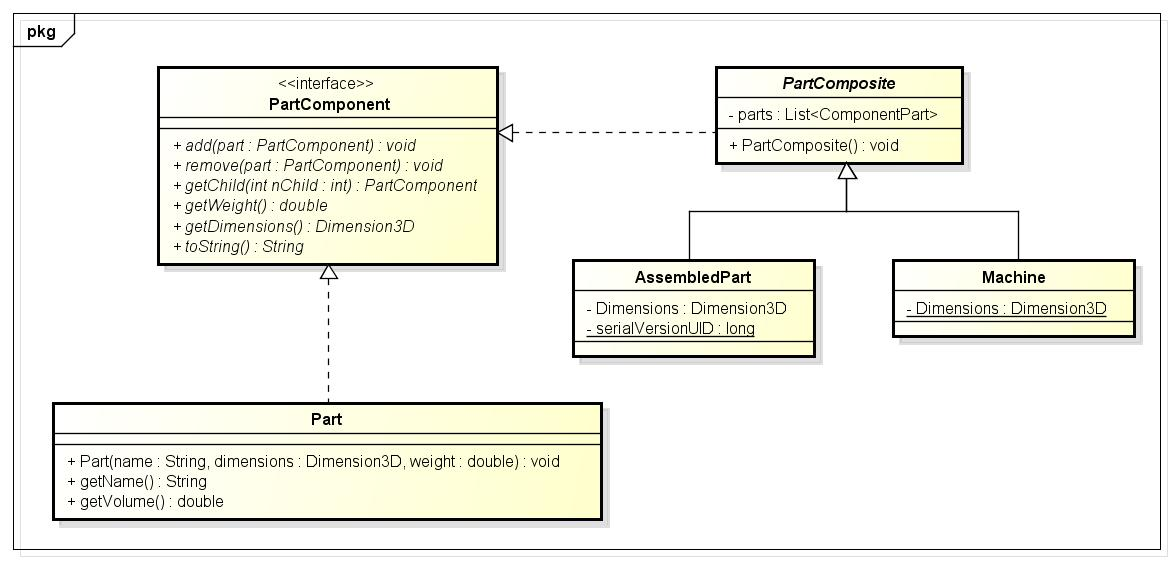
\includegraphics{composite.jpg}
\caption{Composite}
\end{figure}

\subsection{Singleton}\label{singleton}

\subsubsection{Identification}\label{identification-1}

Nous avons identifié la classe \texttt{Config} comme la classe à
transformer en singleton. Il parait logique que notre application ne
puisse avoir qu'une seule instance de cet objet. Les autres classes
n'auraient pas de sens en singleton.

\subsubsection{Implémentation}\label{impluxe9mentation}

Pour transformer cette classe en singleton, voici les changements que
nous avons effectué :

\begin{Shaded}
\begin{Highlighting}[]
\CommentTok{// Constructeur privé afin de ne pas pouvoir le créer}
\CommentTok{// autrement que par "getConfig()"}
\KeywordTok{private} \FunctionTok{Config}\NormalTok{() \{}
   \KeywordTok{this}\NormalTok{.}\FunctionTok{propertyFileName}\NormalTok{ = CONFIG_FILE;}
   \FunctionTok{load}\NormalTok{();}
\NormalTok{\}}

\CommentTok{// Function statique permettant de créer une instance de Config si elle}
\CommentTok{// n'est pas encore existante}
\KeywordTok{public} \DataTypeTok{static}\NormalTok{ Config }\FunctionTok{getConfig}\NormalTok{() \{}
   \KeywordTok{if}\NormalTok{ (Config.}\FunctionTok{instance}\NormalTok{ == }\KeywordTok{null}\NormalTok{) \{}
\NormalTok{      Config.}\FunctionTok{instance}\NormalTok{ = }\KeywordTok{new} \FunctionTok{Config}\NormalTok{();}
\NormalTok{   \}}
   \KeywordTok{return}\NormalTok{ Config.}\FunctionTok{instance}\NormalTok{;}
\NormalTok{\}}

\CommentTok{// Instance unique de notre classe "Config"}
\CommentTok{// De plus, on stocke le nom du fichier sous forme de constante}
\KeywordTok{private} \DataTypeTok{static}\NormalTok{ Config instance = }\KeywordTok{null}\NormalTok{;}
\KeywordTok{private} \DataTypeTok{static} \DataTypeTok{final} \BuiltInTok{String}\NormalTok{ CONFIG_FILE = }\StringTok{"config.properties"}\NormalTok{;}
\end{Highlighting}
\end{Shaded}

De plus, il n'est pas possible de définir le nom de fichier dans la
méthode \texttt{getConfig()}, car cela n'aurait pas de sens. Une fois la
première instance créée avec un certain nom de fichier, le prochain
appel ne prendrait pas en compte un nouveau nom de fichier. C'est
pourquoi nous avons décidé de mettre un nom de fichier en static. Et
également l'application dans son état initial n'a aucun appel au
constructeur avec un nom de fichier spécifié

Nous aurions pu implémenter le singleton en utilisant un énuméré, mais
n'avons pas choisi cette solution, car dans le cas où nous ne faisons
pas appel à cette instance, celle-ci est créée pour rien. Ce problème
est encore plus flagrant dans le cas ou nous avons plus qu'une instance.

\subsubsection{Conclusion}\label{conclusion-1}

Ce pattern nous permet de nous assurer qu'une seule et unique instance
sera disponible. De plus, cette façon de faire permet d'avoir accès à
l'instance à partir de n'importe quel endroit du code (un genre de
variable global en somme). C'est d'ailleurs pour cette dernière raison
que certains programmeurs ne sont pas très enthousiastes concernant ce
patron de conception.

En conclusion, nous pensons que ce patron de conception peut être bien
utile. Cependant il faut l'utiliser avec parcimonie et avoir de bonnes
raisons pour l'utiliser.

\paragraph{Diagramme de classe}\label{diagramme-de-classe-1}

\begin{figure}
\centering
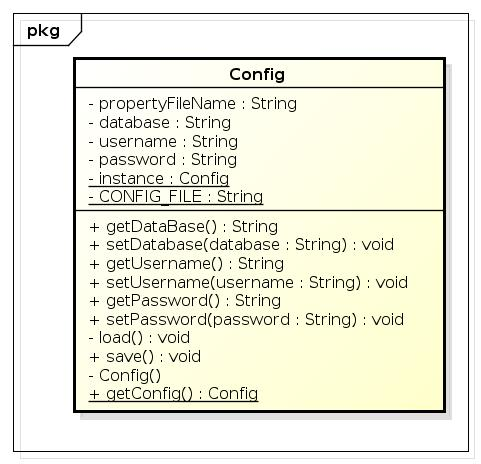
\includegraphics{singleton.jpg}
\caption{Singleton}
\end{figure}

\end{document}
